% Task 3: Salsa20 vs ChaCha20, which one mixes faster. The layouts are from Task3/salsa.py and Task3/chacha.py;
% the quarter rounds are the code of the two modules. The numbers (bits changed) are not shown: that is the task.
\documentclass[12pt,tikz,border=6pt]{standalone}
% Shared preamble of the task figures of Lecture 2 (a copy of Lecture01-RC4/task-figures/common.tex).
% The colours and styles are copied from the preamble of ../main.tex (keep them in sync).
% The ChaCha20 roles take the colours of the ChaCha20 simulator (CryptographySimulators/chacha20),
% so that the README figures and the simulator look the same:
%   key: amber, nonce: blue, counter: green, constants: grey, ciphertext: violet, a change: orange.
\usepackage{lmodern}
\usepackage[T1]{fontenc}
\renewcommand{\familydefault}{\sfdefault}
\usepackage{amsmath,amssymb}
\usepackage{xcolor}
\usepackage{fontawesome5}
\usetikzlibrary{arrows.meta, calc, positioning, fit, decorations.pathreplacing, decorations.pathmorphing, backgrounds}

% ---------- template ----------
\definecolor{DeepBlue}{HTML}{283593}
\definecolor{AccentOrange}{HTML}{EB5A14}
\definecolor{LightGray}{HTML}{F5F6FA}
% ---------- actors and categories (S1 to S6) ----------
\definecolor{sIndigo}{HTML}{5C6BC0}   % the sender
\definecolor{sPink}{HTML}{EC407A}     % the attacker
\definecolor{sViolet}{HTML}{7E57C2}   % plaintext
\definecolor{sAmber}{HTML}{FFB300}    % key and keystream
\definecolor{sTeal}{HTML}{26A69A}     % the receiver
\definecolor{sBrown}{HTML}{8D6E63}    % ciphertext
\definecolor{sPinkText}{HTML}{C2185B}
\definecolor{sAmberText}{HTML}{A06A00}
\definecolor{sTealText}{HTML}{00796B}
% ---------- actions and results ----------
\definecolor{aExec}{HTML}{43A047}
\definecolor{aRead}{HTML}{1E88E5}
\definecolor{aWrite}{HTML}{E53935}
% ---------- neutral ----------
\definecolor{nInk}{HTML}{37474F}
\definecolor{nLine}{HTML}{90A4AE}
\definecolor{nLight}{HTML}{CFD8DC}
\definecolor{nFill}{HTML}{ECEFF1}
\definecolor{nIdle}{HTML}{E0E0E0}

% ---------- TikZ styles (as in main.tex; byte cells a little larger for the web) ----------
\tikzset{
  hw/.style={draw=nLine, thick, fill=nFill, text=nInk, rounded corners=3pt, align=center, inner sep=4pt},
  hwmain/.style={draw=nInk, thick, fill=nInk, text=white, rounded corners=3pt, align=center, inner sep=4pt},
  cell/.style={draw=nLine, thick, fill=white, text=nInk, font=\ttfamily\small},
  cellfree/.style={cell, dashed, draw=nLight},
  container/.style={draw=nLine, thick, dashed, rounded corners=5pt},
  actor/.style={fill=#1, draw=#1, text=white, rounded corners=3pt, align=center, font=\small\bfseries, inner sep=5pt},
  actorlight/.style={fill=#1!15, draw=#1, thick, text=nInk, rounded corners=3pt, align=center, inner sep=5pt},
  data/.style={-{Stealth}, very thick, nInk},
  flow/.style={-{Stealth}, very thick, DeepBlue},
  annot/.style={draw=AccentOrange, line width=1.6pt, rounded corners=3pt},
  byte/.style={draw=nLine, thick, fill=white, text=nInk, font=\ttfamily\small,
    minimum width=0.8cm, minimum height=0.62cm, inner sep=1pt, rounded corners=1.5pt},
  ptb/.style={byte, fill=white, draw=nInk},   % plaintext: neutral here, violet is the ciphertext
  ksb/.style={byte, fill=sAmber!25, draw=sAmber},
  rowlabel/.style={font=\small\bfseries, text=nInk, anchor=east},
  note/.style={font=\small, text=nInk},
  bigxor/.style={circle, draw=nInk, very thick, fill=white, inner sep=0pt, minimum size=0.8cm, font=\Large},
  radio/.style={-{Stealth}, very thick, nInk, decorate,
    decoration={snake, amplitude=1.2pt, segment length=7pt, post length=4pt}},
  % a white card behind the whole figure, so that it stays readable in a dark theme
  card/.style={show background rectangle, background rectangle/.style={fill=white, draw=none}, inner frame sep=8pt},
}
% a row of bytes: \byterow{x of the first cell}{y}{style}{list of values}{step between cells}
\newcommand{\byterow}[5]{%
  \expandafter\def\expandafter\brlist\expandafter{#4}%
  \foreach \v [count=\k from 0] in \brlist {
    \node[#3] at ({#1+#5*\k},#2) {\v};
  }}
% the generator / cipher box: dark, with cogs. \cogbox{name}{position}{label}{width}
\newcommand{\cogbox}[4]{%
  \node[hwmain, minimum width=#4, minimum height=1.3cm] (#1) at (#2) {};
  \node[text=white, font=\Large] at ([yshift=0.22cm]#1.center) {\faCogs};
  \node[text=white, font=\small\bfseries] at ([yshift=-0.32cm]#1.center) {#3};}
\newcommand{\ok}{\textcolor{aExec}{\faCheck}}
\newcommand{\nok}{\textcolor{aWrite}{\faTimes}}
\newcommand{\badge}[1]{\tikz[baseline=(b.base)]\node[circle,fill=AccentOrange,text=white,
  inner sep=1.5pt,font=\bfseries\footnotesize] (b) {#1};}

% ---------- ChaCha20 roles (the colours of the ChaCha20 simulator) ----------
\definecolor{rKey}{HTML}{E2A60E}    \definecolor{rKeyBg}{HTML}{FDF3DC}
\definecolor{rNonce}{HTML}{2F6FDB}  \definecolor{rNonceBg}{HTML}{E5EDFB}
\definecolor{rCtr}{HTML}{2FA84F}    \definecolor{rCtrBg}{HTML}{E3F4E8}
\definecolor{rConst}{HTML}{BCC4CC}  \definecolor{rConstBg}{HTML}{EEF1F4}
\definecolor{rCt}{HTML}{8A5CD8}     \definecolor{rCtBg}{HTML}{F1EAFD}
\definecolor{rKeyText}{HTML}{9A6B00}
\definecolor{rNonceText}{HTML}{1F55B5}
\definecolor{rCtrText}{HTML}{1E7E4F}
\definecolor{rCtText}{HTML}{6A3FB8}
\definecolor{rChg}{HTML}{D9621C}
\tikzset{
  keyb/.style={byte, fill=rKeyBg, draw=rKey},
  nonceb/.style={byte, fill=rNonceBg, draw=rNonce},
  ctrb/.style={byte, fill=rCtrBg, draw=rCtr},
  ctb/.style={byte, fill=rCtBg, draw=rCt},
  chg/.style={byte, fill=AccentOrange!18, draw=AccentOrange, line width=1.4pt, font=\ttfamily\small\bfseries},
  unk/.style={byte, fill=white, dashed, text=nInk},
  inbox/.style={draw=#1, thick, fill=#1!12, text=nInk, rounded corners=3pt, align=center, inner sep=5pt},
}

\begin{document}
\pagecolor{white}
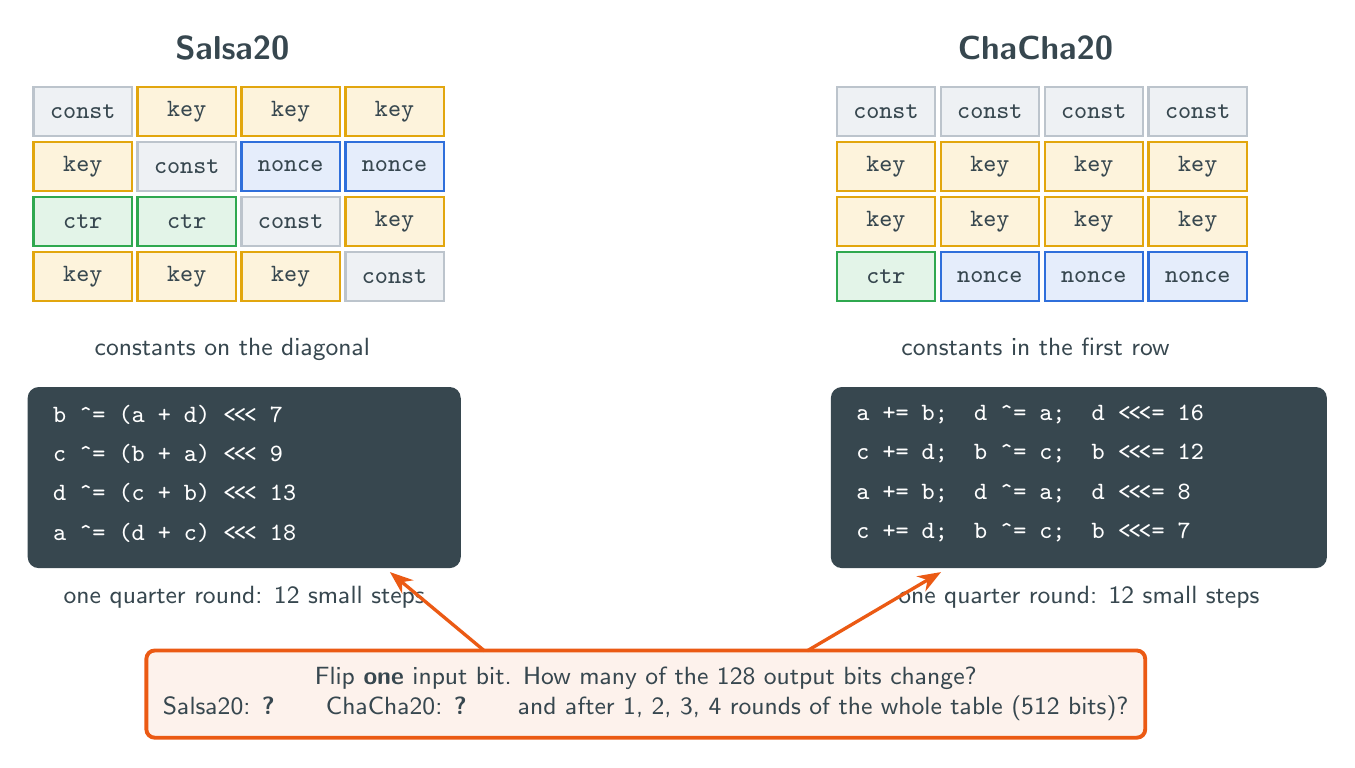
\begin{tikzpicture}[>=Stealth]
  \tikzset{w/.style={draw=#1, thick, fill=#1Bg, minimum width=1.25cm, minimum height=0.62cm, font=\ttfamily\small, text=nInk}}
  % ---------- the two tables ----------
  \foreach \name/\x/\lay in {Salsa20/0/{c,k,k,k,k,c,n,n,t,t,c,k,k,k,k,c}, ChaCha20/10.2/{c,c,c,c,k,k,k,k,k,k,k,k,t,n,n,n}} {
    \node[font=\large\bfseries, text=nInk] at ({\x+2.0},1.0) {\name};
    \foreach \r [count=\i from 0] in \lay {
      \pgfmathtruncatemacro{\row}{\i/4}\pgfmathtruncatemacro{\col}{mod(\i,4)}
      \if\r c\node[w=rConst] at ({\x+0.1+1.32*\col},{-0.7*\row+0.2}) {const};\fi
      \if\r k\node[w=rKey] at ({\x+0.1+1.32*\col},{-0.7*\row+0.2}) {key};\fi
      \if\r n\node[w=rNonce] at ({\x+0.1+1.32*\col},{-0.7*\row+0.2}) {nonce};\fi
      \if\r t\node[w=rCtr] at ({\x+0.1+1.32*\col},{-0.7*\row+0.2}) {ctr};\fi
    }
  }
  \node[note, anchor=north] at (2.0,-2.55) {constants on the diagonal};
  \node[note, anchor=north] at (12.2,-2.55) {constants in the first row};
  % ---------- the two quarter rounds ----------
  \foreach \x/\l [count=\j from 0] in {0/{b \textasciicircum= (a + d) <\kern-1pt<\kern-1pt< 7,
                                          c \textasciicircum= (b + a) <\kern-1pt<\kern-1pt< 9,
                                          d \textasciicircum= (c + b) <\kern-1pt<\kern-1pt< 13,
                                          a \textasciicircum= (d + c) <\kern-1pt<\kern-1pt< 18}} {
    \foreach \t [count=\k from 0] in \l \node[font=\ttfamily\small, text=white, anchor=west] at (-0.4,{-3.65-0.5*\k}) {\t};
  }
  \begin{scope}[on background layer]
    \fill[nInk, rounded corners=4pt] (-0.6,-3.3) rectangle (4.9,-5.6);
    \fill[nInk, rounded corners=4pt] (9.6,-3.3) rectangle (15.9,-5.6);
  \end{scope}
  \foreach \t [count=\k from 0] in {a += b;\ \ d \textasciicircum= a;\ \ d <\kern-1pt<\kern-1pt<= 16,
                                    c += d;\ \ b \textasciicircum= c;\ \ b <\kern-1pt<\kern-1pt<= 12,
                                    a += b;\ \ d \textasciicircum= a;\ \ d <\kern-1pt<\kern-1pt<= 8,
                                    c += d;\ \ b \textasciicircum= c;\ \ b <\kern-1pt<\kern-1pt<= 7}
    \node[font=\ttfamily\small, text=white, anchor=west] at (9.8,{-3.65-0.5*\k}) {\t};
  \node[note, anchor=north] at (2.15,-5.7) {one quarter round: 12 small steps};
  \node[note, anchor=north] at (12.75,-5.7) {one quarter round: 12 small steps};
  % ---------- the question ----------
  \node[draw=AccentOrange, line width=1.4pt, rounded corners=3pt, fill=AccentOrange!8, font=\small, text=nInk, align=center, inner sep=6pt]
    at (7.25,-7.2) {Flip \textbf{one} input bit. How many of the 128 output bits change?\\
                    Salsa20: \textbf{?}\qquad ChaCha20: \textbf{?}\qquad and after 1, 2, 3, 4 rounds of the whole table (512 bits)?};
  \draw[->, very thick, AccentOrange] (5.2,-6.65) -- (4.0,-5.65);
  \draw[->, very thick, AccentOrange] (9.3,-6.65) -- (11.0,-5.65);
\end{tikzpicture}
\end{document}
